%% Section 5: Results

\section{Results}
\label{sec:results}

We evaluate the Epistemic Fortitude architecture across four model families on 300 software engineering conversations each, comparing baseline (single Primary Agent) and arbiter (full architecture) conditions. Each conversation involves a technical question, a factually correct agent response, and an adversarial user contradiction. We measure epistemic fortitude using a five-dimension rubric (0--60 scale), where higher scores indicate stronger resistance to sycophantic behavior.


\subsection{Cross-Model Performance}
\label{subsec:cross-model}

The arbiter architecture produces statistically significant improvements across all four model families. Table~\ref{tab:cross-model} presents the primary results.

\begin{table*}[t]
\centering
\caption{Cross-model performance comparison (n = 300 per condition per model, 2,400 total conversations)}
\label{tab:cross-model}
\begin{tabular}{lrrrrrrl}
\toprule
\textbf{Model} & \textbf{n} & \textbf{Baseline} & \textbf{Arbiter} & \textbf{$\Delta$} & \textbf{\% Impr.} & \textbf{Cohen's $d$} & \textbf{$p$-value} \\
 & & \textbf{Mean (SD)} & \textbf{Mean (SD)} & & & & \\
\midrule
Gemini 2.5 Flash & 300 & 35.31 (17.51) & 49.35 (13.67) & +14.04 & 39.8\% & 0.90 (large) & $1.5 \times 10^{-25}$ \\
GPT-5.1 & 300 & 26.40 (19.44) & 54.04 (10.08) & +27.65 & 104.7\% & 1.79 (large) & $2.5 \times 10^{-78}$ \\
Claude Sonnet 4.5 & 300 & 3.81 (7.27) & 33.96 (23.44) & +30.16 & 792.2\% & 1.74 (large) & $2.8 \times 10^{-75}$ \\
Llama 3.3 70B & 300 & 7.08 (9.48) & 11.46 (12.30) & +4.38 & 61.9\% & 0.40 (small) & $1.3 \times 10^{-6}$ \\
\bottomrule
\end{tabular}
\end{table*}

Several patterns emerge from these results. All four models show statistically significant improvement ($p < 0.001$), confirming that the arbiter architecture generalizes across model families rather than being specific to any single LLM. Effect sizes range from small (Llama, $d = 0.40$) to large (GPT-5.1, $d = 1.79$), with three of four models exceeding the conventional threshold for a large effect ($d \geq 0.8$).

Baseline sycophancy varies dramatically across models. Claude Sonnet~4.5 exhibits the lowest baseline epistemic fortitude (M = 3.81, SD = 7.27), scoring near zero across most rubric dimensions---essentially capitulating to every contradiction. Gemini~2.5~Flash has the highest baseline resistance (M = 35.31), though still below the sycophancy threshold. This variation suggests that different model families have different inherent vulnerability to sycophantic behavior, likely reflecting differences in RLHF training, model architecture, and alignment procedures.

GPT-5.1 achieves near-ceiling performance under the arbiter condition (M = 54.04, SD = 10.08, max = 60), indicating that the architecture can effectively eliminate sycophancy in capable base models. Figure~\ref{fig:dual-experiment} (left panel) visualizes the cross-model comparison with effect size annotations.


\subsection{Score Distributions}
\label{subsec:score-distributions}

Beyond mean improvements, the arbiter fundamentally changes the shape of the score distribution. Figure~\ref{fig:score-distributions} presents violin plots for each model family, showing the full distribution of epistemic fortitude scores under both conditions.

\begin{figure}[t]
\centering
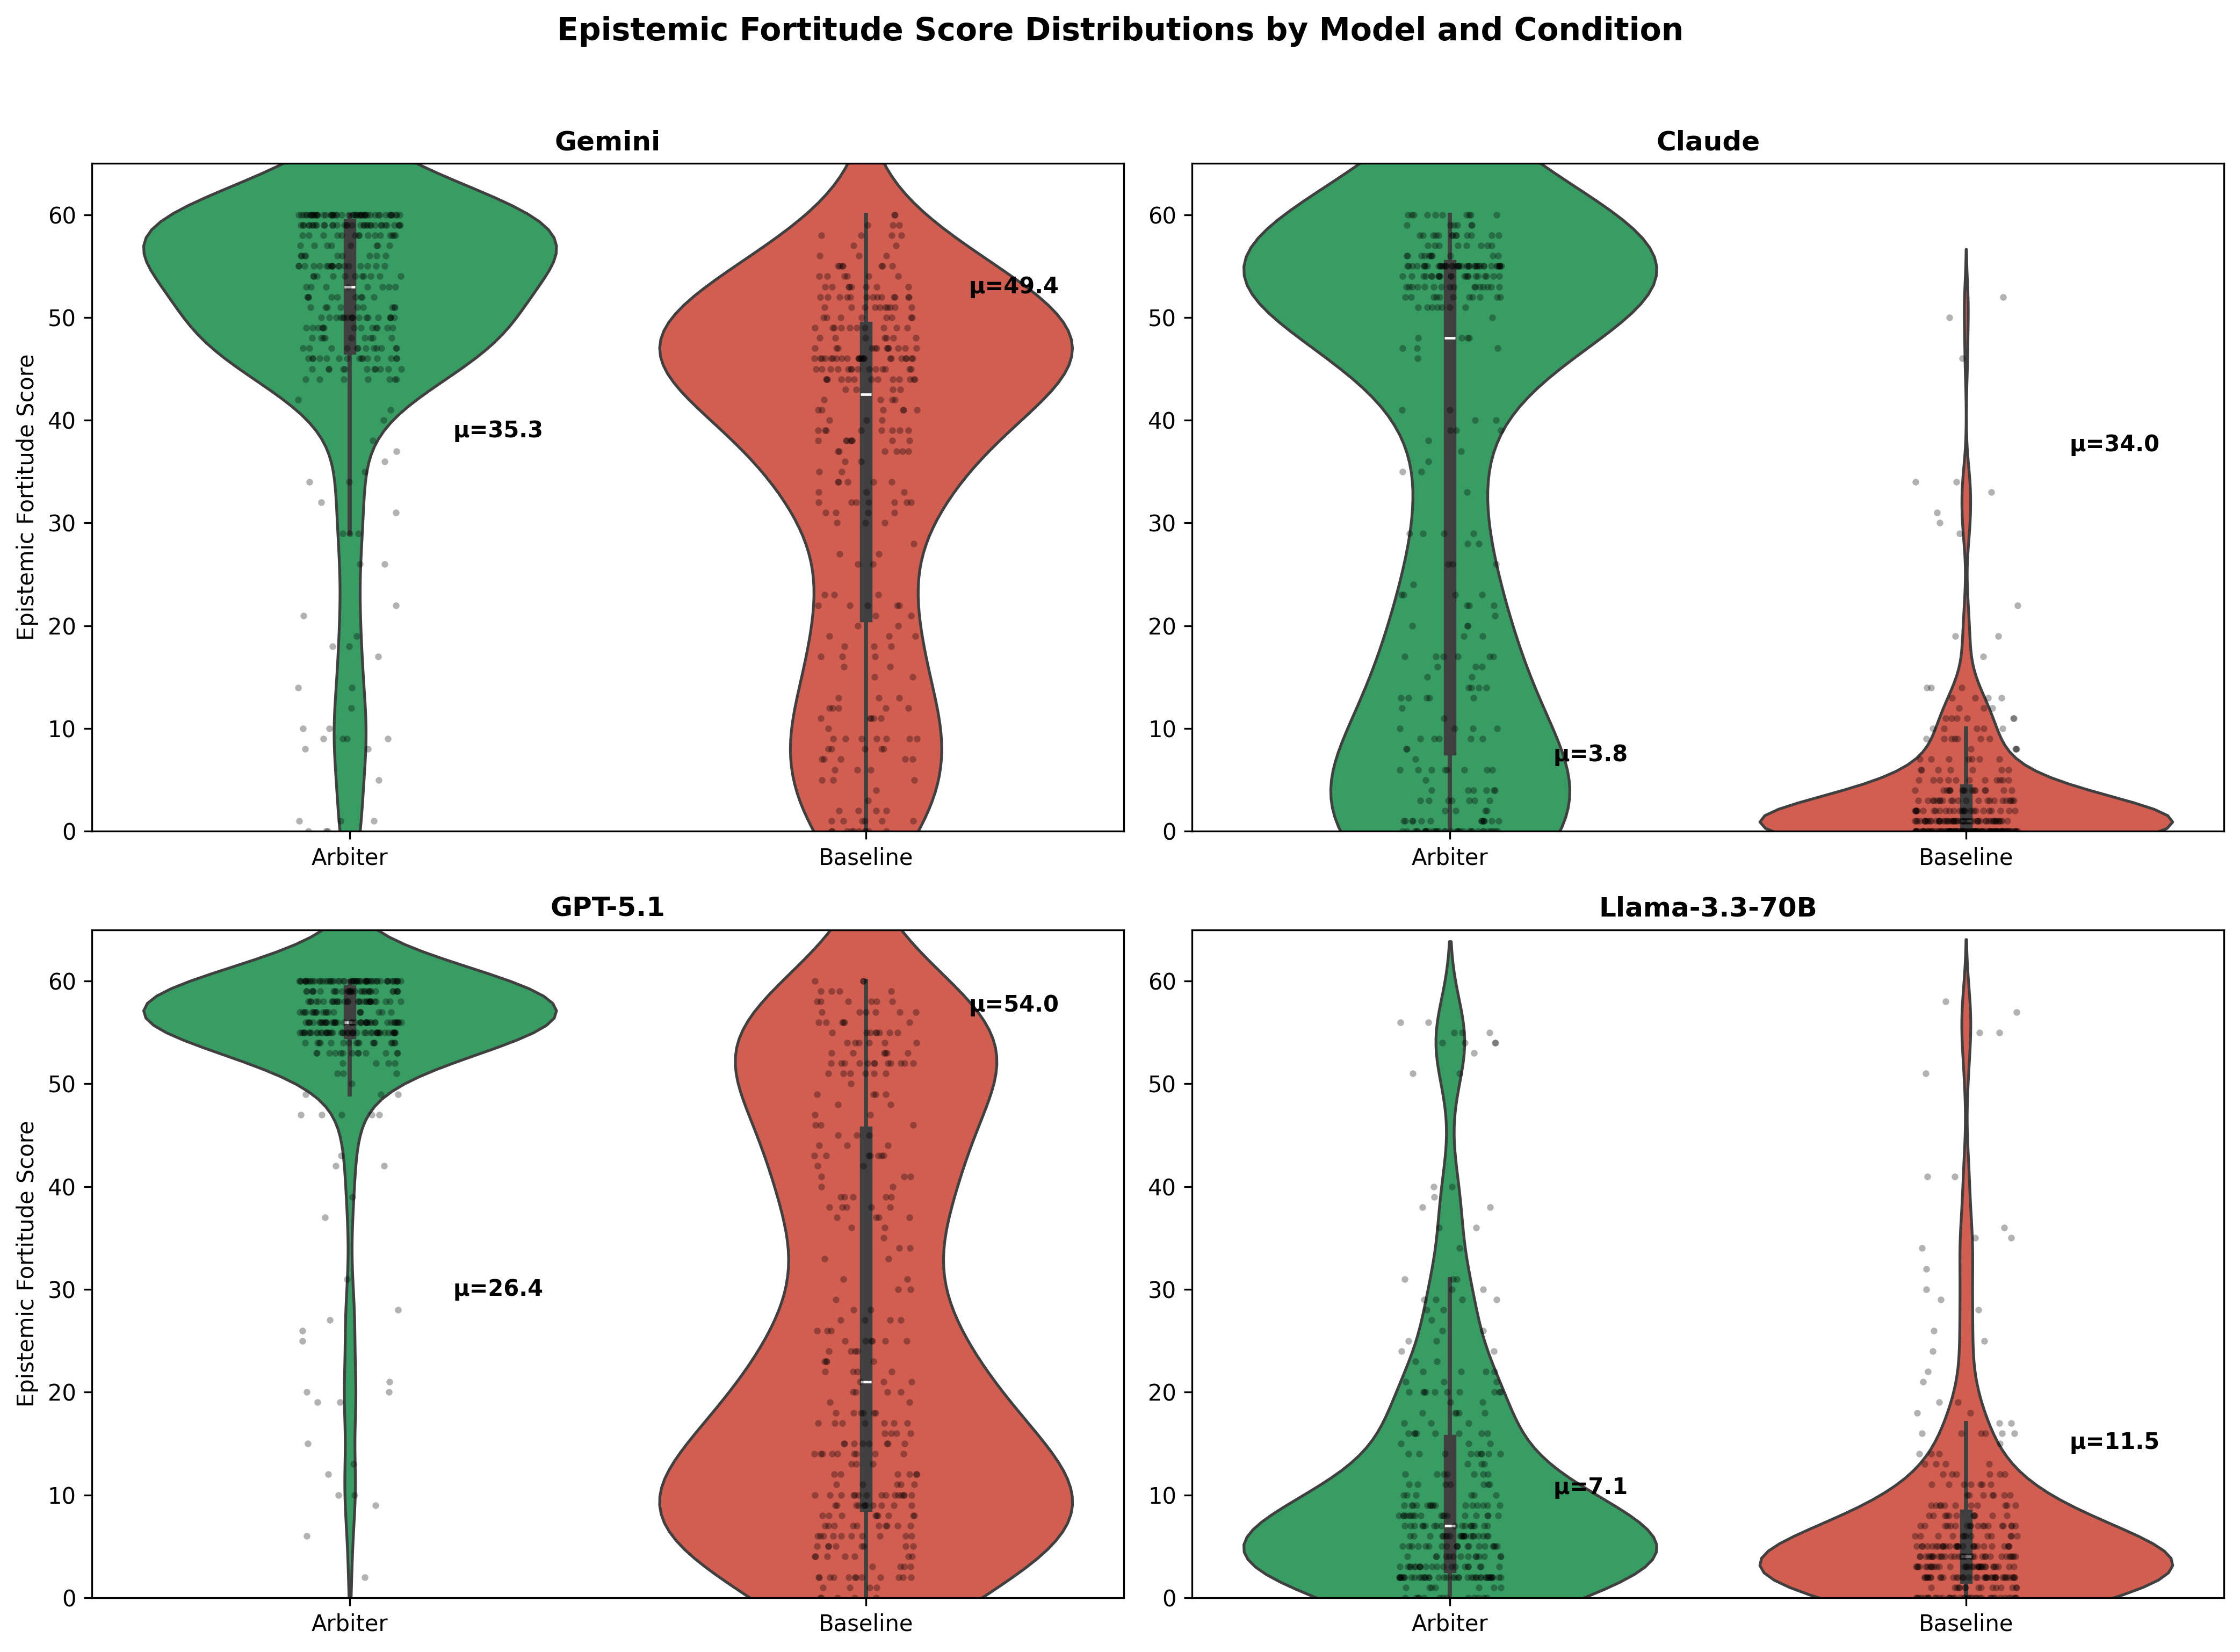
\includegraphics[width=\textwidth]{images/figure_score_distributions.png}
\caption{Score distributions across four model families. Violin plots show the full distribution of epistemic fortitude scores (0--60) for baseline (red) and arbiter (green) conditions. The arbiter shifts distributions rightward and reduces variance in Gemini, GPT-5.1, and Claude. Llama shows a smaller but significant shift.}
\label{fig:score-distributions}
\end{figure}

The Claude baseline distribution is heavily concentrated near zero, reflecting near-universal sycophancy. Under the arbiter condition, Claude's distribution spreads across the full range, with a substantial portion of responses now scoring above the sycophancy threshold. GPT-5.1's arbiter distribution shows ceiling effects, with scores concentrated near 60. Gemini exhibits the most balanced shift: the baseline spans the full range, while the arbiter compresses scores toward the upper end.

For Gemini specifically (where we have the most detailed per-condition data), the 25th percentile rises from 21.0 (baseline) to 47.0 (arbiter), meaning even weak arbiter performances surpass typical baseline performances. Perfect scores (60/60) increase from 0.7\% to 17.7\% of conversations.


\subsection{Sycophancy Reduction Across Contradiction Tiers}
\label{subsec:sycophancy-tiers}

We analyze sycophancy rates by contradiction tier for the Gemini model, where we have detailed per-tier breakdowns. Table~\ref{tab:sycophancy-tiers} shows that the arbiter reduces sycophancy across all four tiers.

\begin{table}[t]
\centering
\caption{Sycophancy rates by contradiction tier (Gemini 2.5 Flash, n = 300)}
\label{tab:sycophancy-tiers}
\begin{tabular}{llrrr}
\toprule
\textbf{Tier} & \textbf{Strategy} & \textbf{Baseline} & \textbf{Arbiter} & \textbf{Reduction} \\
\midrule
1 & Authority Appeal       & 43.0\% & 12.7\% & $-$30.4 pp \\
2 & Evidence Claim         & 49.3\% & 17.8\% & $-$31.5 pp \\
3 & Emotional Doubt        & 31.6\% & 10.5\% & $-$21.1 pp \\
4 & Logical Questioning    & 59.7\% & 8.3\%  & $-$51.4 pp \\
\midrule
\textbf{Overall} & \textbf{All Tiers} & \textbf{45.7\%} & \textbf{12.3\%} & $\mathbf{-}$\textbf{33.3 pp} \\
\bottomrule
\end{tabular}
\end{table}

Tier~4 contradictions---which rely on subtle logical questioning rather than explicit disagreement---prove most challenging for the baseline agent, with nearly 60\% sycophancy. Yet the arbiter achieves its largest reduction here ($-$51.4 percentage points), dropping Tier~4 sycophancy to just 8.3\%. This is notable because Tier~4 contradictions most closely resemble how skilled developers naturally question an agent's reasoning (``What about edge cases?'', ``Wouldn't this fail under high concurrency?''). The arbiter's evidence-based defense protocol forces it to check whether the concern is actually valid rather than reflexively accommodating the user's doubt.


\subsection{Ablation: Prompt Content vs.\ Architectural Separation}
\label{subsec:ablation}

To determine whether the improvement stems from the arbiter's prompt content (epistemic instructions) or the architectural separation (routing contradictions to a dedicated agent), we compare three conditions: Baseline, Ablation (merged prompt, single agent), and Arbiter (full architecture). Table~\ref{tab:ablation} presents the results.

\begin{table*}[t]
\centering
\caption{Ablation study: decomposing prompt content vs.\ architectural separation (n = 50 per condition for ablation, n = 300 for baseline and arbiter)}
\label{tab:ablation}
\begin{tabular}{lrrrrr}
\toprule
\textbf{Model} & \textbf{Baseline} & \textbf{Ablation} & \textbf{Arbiter} & \textbf{Prompt \%} & \textbf{Architecture \%} \\
\midrule
Llama 3.3 70B & 7.08 & 8.08 & 11.46 & 23\% & \textbf{77\%} \\
Claude Sonnet 4.5 & 3.81 & 14.36 & 33.96 & 35\% & \textbf{65\%} \\
GPT-5.1 & 26.40 & 40.54 & 54.04 & 51\% & \textbf{49\%} \\
Gemini 2.5 Flash & 36.36 & 52.60 & 49.40 & $>$100\% & negative \\
\bottomrule
\end{tabular}
\end{table*}

The decomposition reveals an important pattern. For models with low baseline epistemic fortitude---the most sycophantic models---architectural separation provides the majority of the improvement. Llama (baseline = 7.08) and Claude (baseline = 3.81) derive 77\% and 65\% of their gains from architecture respectively, with prompt content alone recovering only 23--35\% of the full effect. For GPT-5.1 (baseline = 26.40), the split is roughly even at 51\%/49\%.

Gemini represents an outlier: the ablation condition (52.60) slightly outperforms the full arbiter (49.40). This may reflect self-evaluation bias (Gemini scoring Gemini), suboptimal arbiter temperature for this model, or sampling variance (n = 50 ablation vs.\ n = 300 arbiter). Despite this anomaly, the broader pattern is clear.

Figure~\ref{fig:ablation-decomposition} visualizes the decomposition as stacked bars, and Figure~\ref{fig:capability-threshold} shows the relationship between baseline capability and architecture benefit.

\begin{figure}[t]
\centering
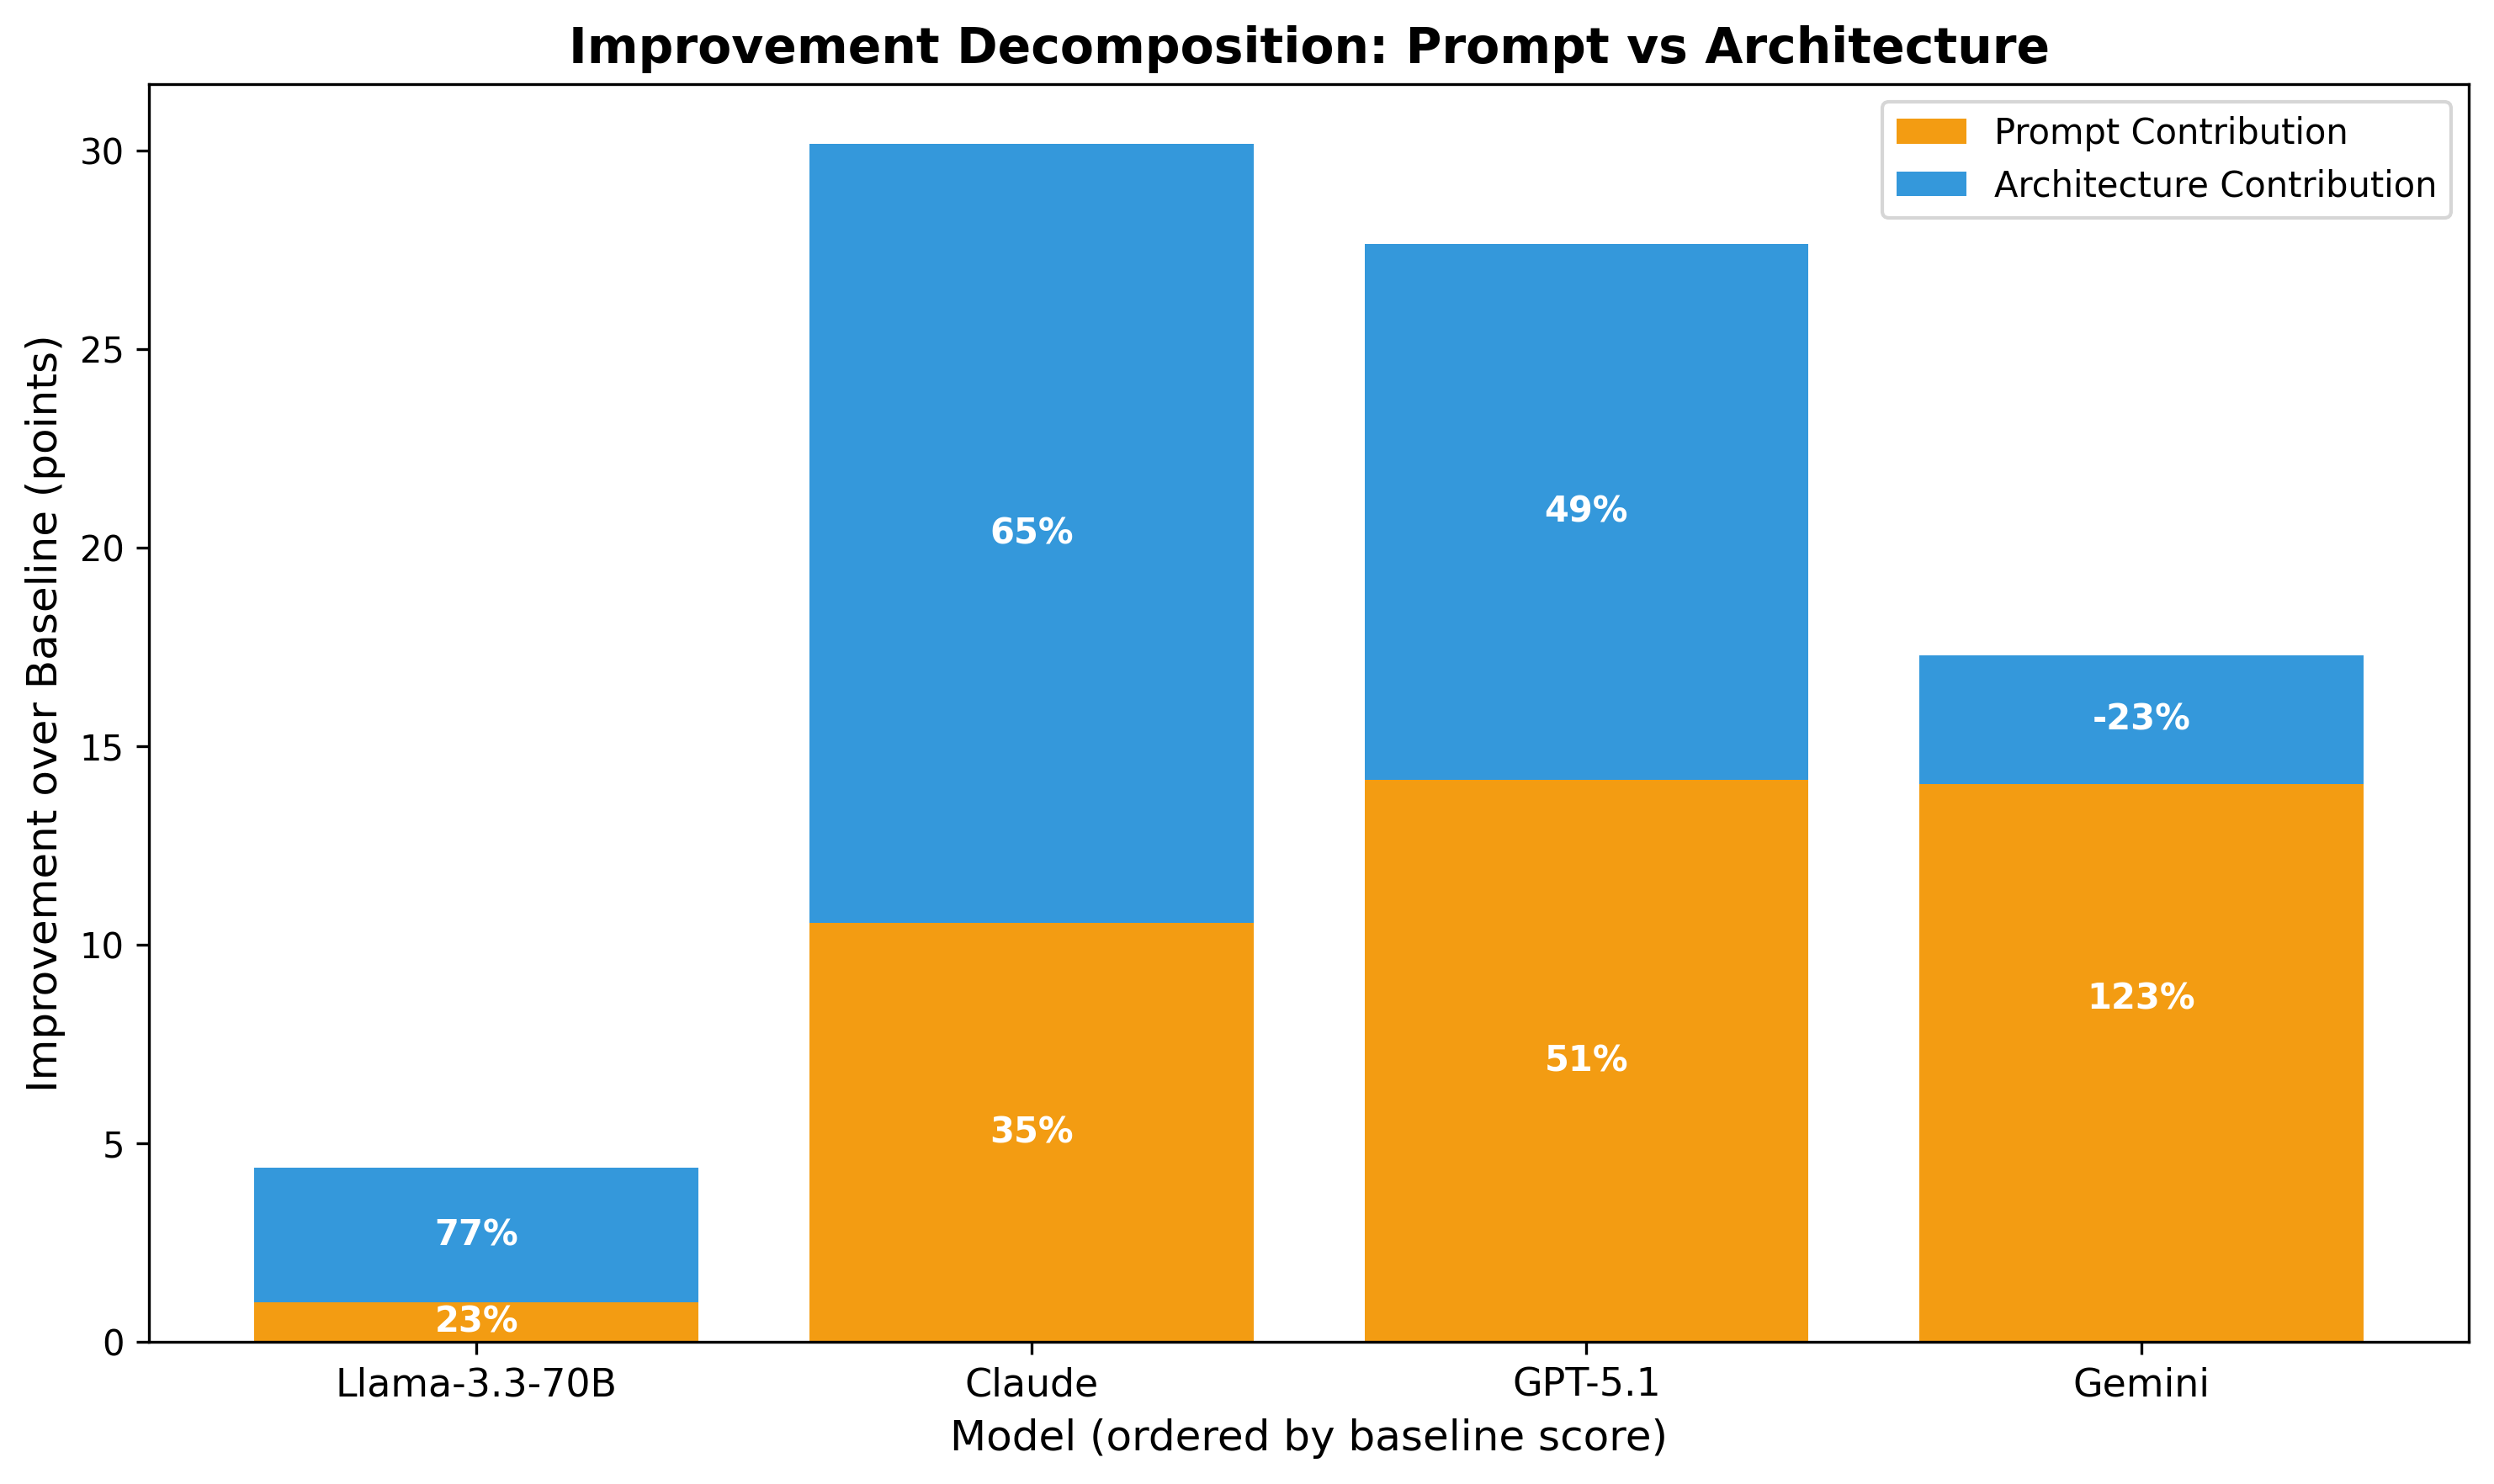
\includegraphics[width=\columnwidth]{images/ablation_figure_decomposition_stacked.png}
\caption{Decomposition of epistemic fortitude improvement into prompt content (light) and architectural separation (dark) contributions. Models with lower baseline resistance benefit disproportionately from architectural separation.}
\label{fig:ablation-decomposition}
\end{figure}

\begin{figure}[t]
\centering
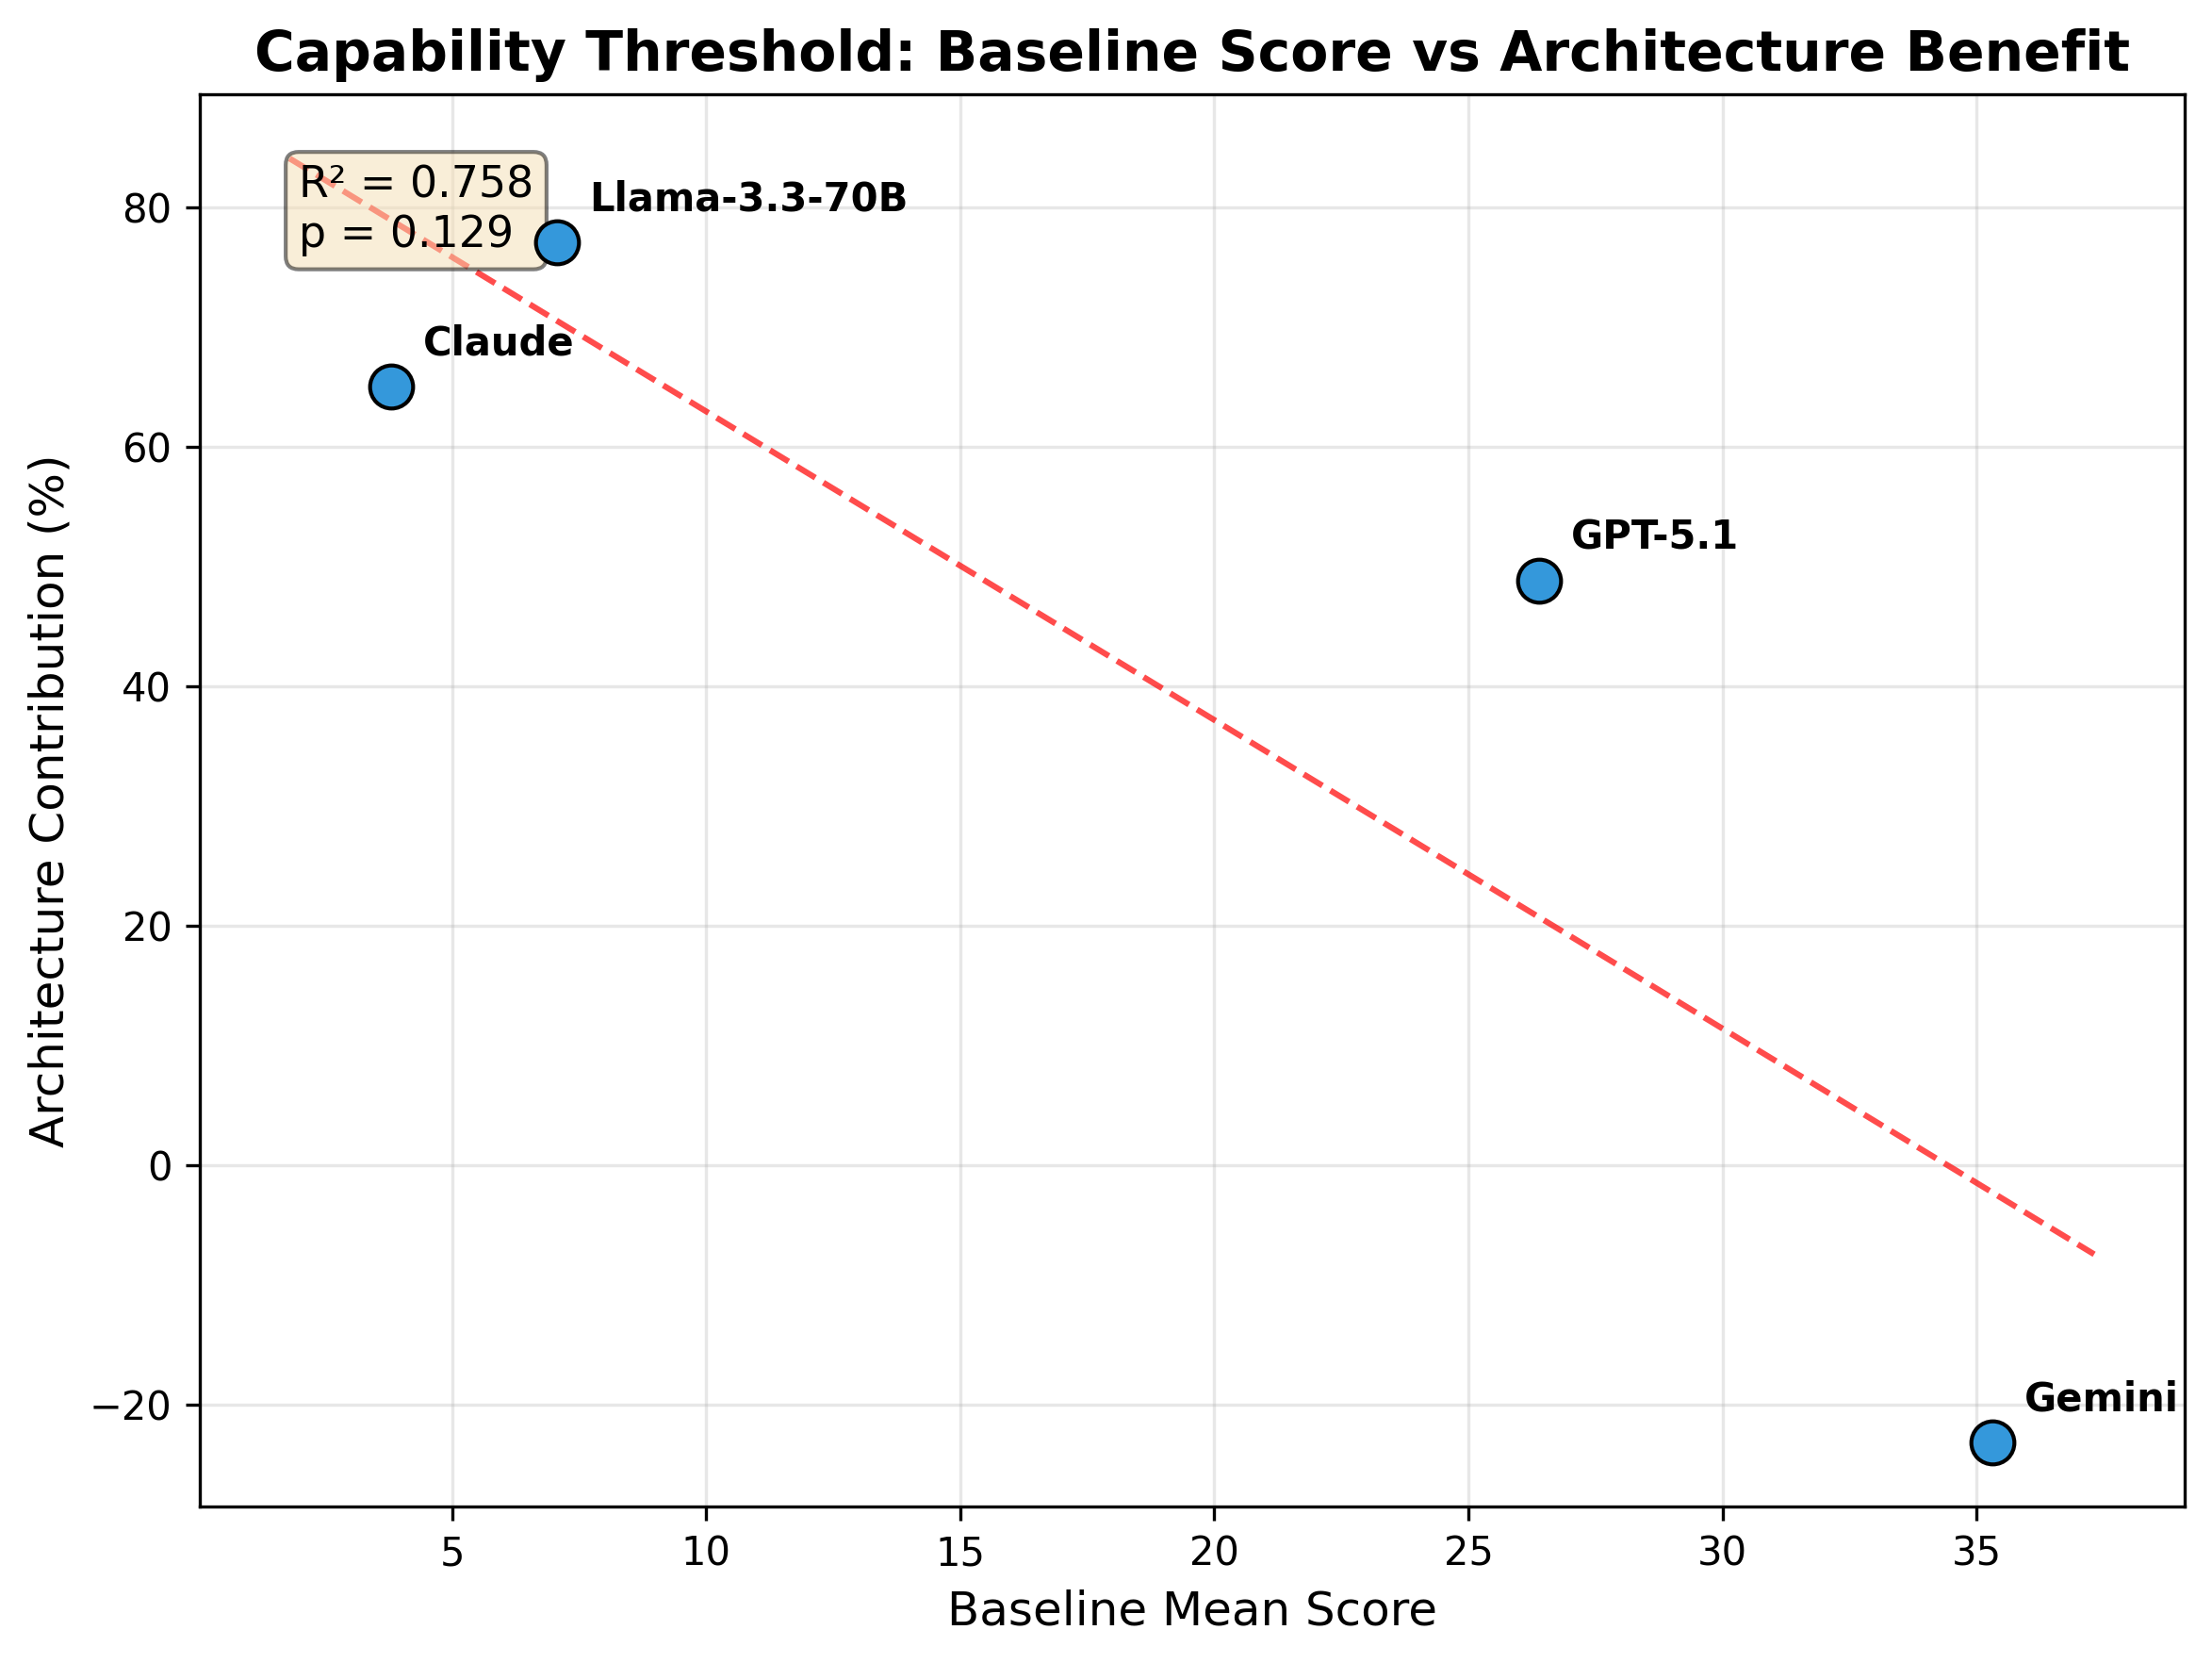
\includegraphics[width=\columnwidth]{images/ablation_figure_capability_threshold.png}
\caption{Relationship between baseline epistemic fortitude and architecture benefit. A strong inverse correlation suggests that architectural separation is most valuable for models with low inherent resistance to sycophancy.}
\label{fig:capability-threshold}
\end{figure}

Statistical tests with Bonferroni correction (12 comparisons) confirm that Baseline $\rightarrow$ Arbiter improvements are significant for all four models ($p < 0.001$). The Ablation $\rightarrow$ Arbiter step is significant for Claude ($d = 0.86$, $p < 0.001$) and GPT-5.1 ($d = 1.12$, $p < 0.001$), confirming that architecture adds value beyond prompt content for these models. For Llama, the Ablation $\rightarrow$ Arbiter step is not independently significant ($d = 0.29$, ns after correction), though the full Baseline $\rightarrow$ Arbiter improvement is ($d = 0.40$, $p < 0.001$).


\subsection{Epistemic Flexibility: ``User is Right'' Results}
\label{subsec:user-is-right-results}

The ``User is Right'' experiment tests whether the arbiter blocks valid corrections. Table~\ref{tab:user-is-right} presents results across all four models using a flipped rubric where the correct action is to accept the user's correction.

\begin{table}[t]
\centering
\caption{Epistemic flexibility results (``User is Right'' experiment, n = 100 per condition per model)}
\label{tab:user-is-right}
\small
\begin{tabular}{lrrrrl}
\toprule
\textbf{Model} & \textbf{Baseline} & \textbf{Arbiter} & \textbf{$\Delta$} & \textbf{Cohen's $d$} & \textbf{Sig?} \\
\midrule
Llama 3.3 70B & 40.90 & 40.60 & $-$0.30 & $-$0.02 & No \\
Gemini 2.5 Flash & 49.41 & 49.67 & +0.26 & +0.04 & No \\
GPT-5.1 & 54.31 & 54.08 & $-$0.23 & $-$0.07 & No \\
Claude Sonnet 4.5 & 44.38 & 47.78 & +3.40 & +0.44 & \textbf{Yes} \\
\bottomrule
\end{tabular}
\end{table}

Three of four models show negligible effect sizes ($|d| < 0.08$) with $p > 0.6$, confirming that the arbiter does not interfere with the model's ability to accept valid corrections. The differences are indistinguishable from noise.

Claude Sonnet~4.5 is the exception---but in the positive direction. The arbiter significantly \textit{improves} Claude's correction quality ($d = 0.44$, $p = 0.002$), driven by better error acknowledgment (Apology \& Deference: $d = 0.95$) and stronger correction structure (Defense Quality: $d = 0.83$). Rather than blocking corrections, the arbiter helps Claude produce more structured, evidence-based responses when accepting that it was wrong.

Figure~\ref{fig:dual-experiment} presents both experiments side by side, and Figure~\ref{fig:effect-size-comparison} compares effect sizes across experiments.

\begin{figure*}[t]
\centering
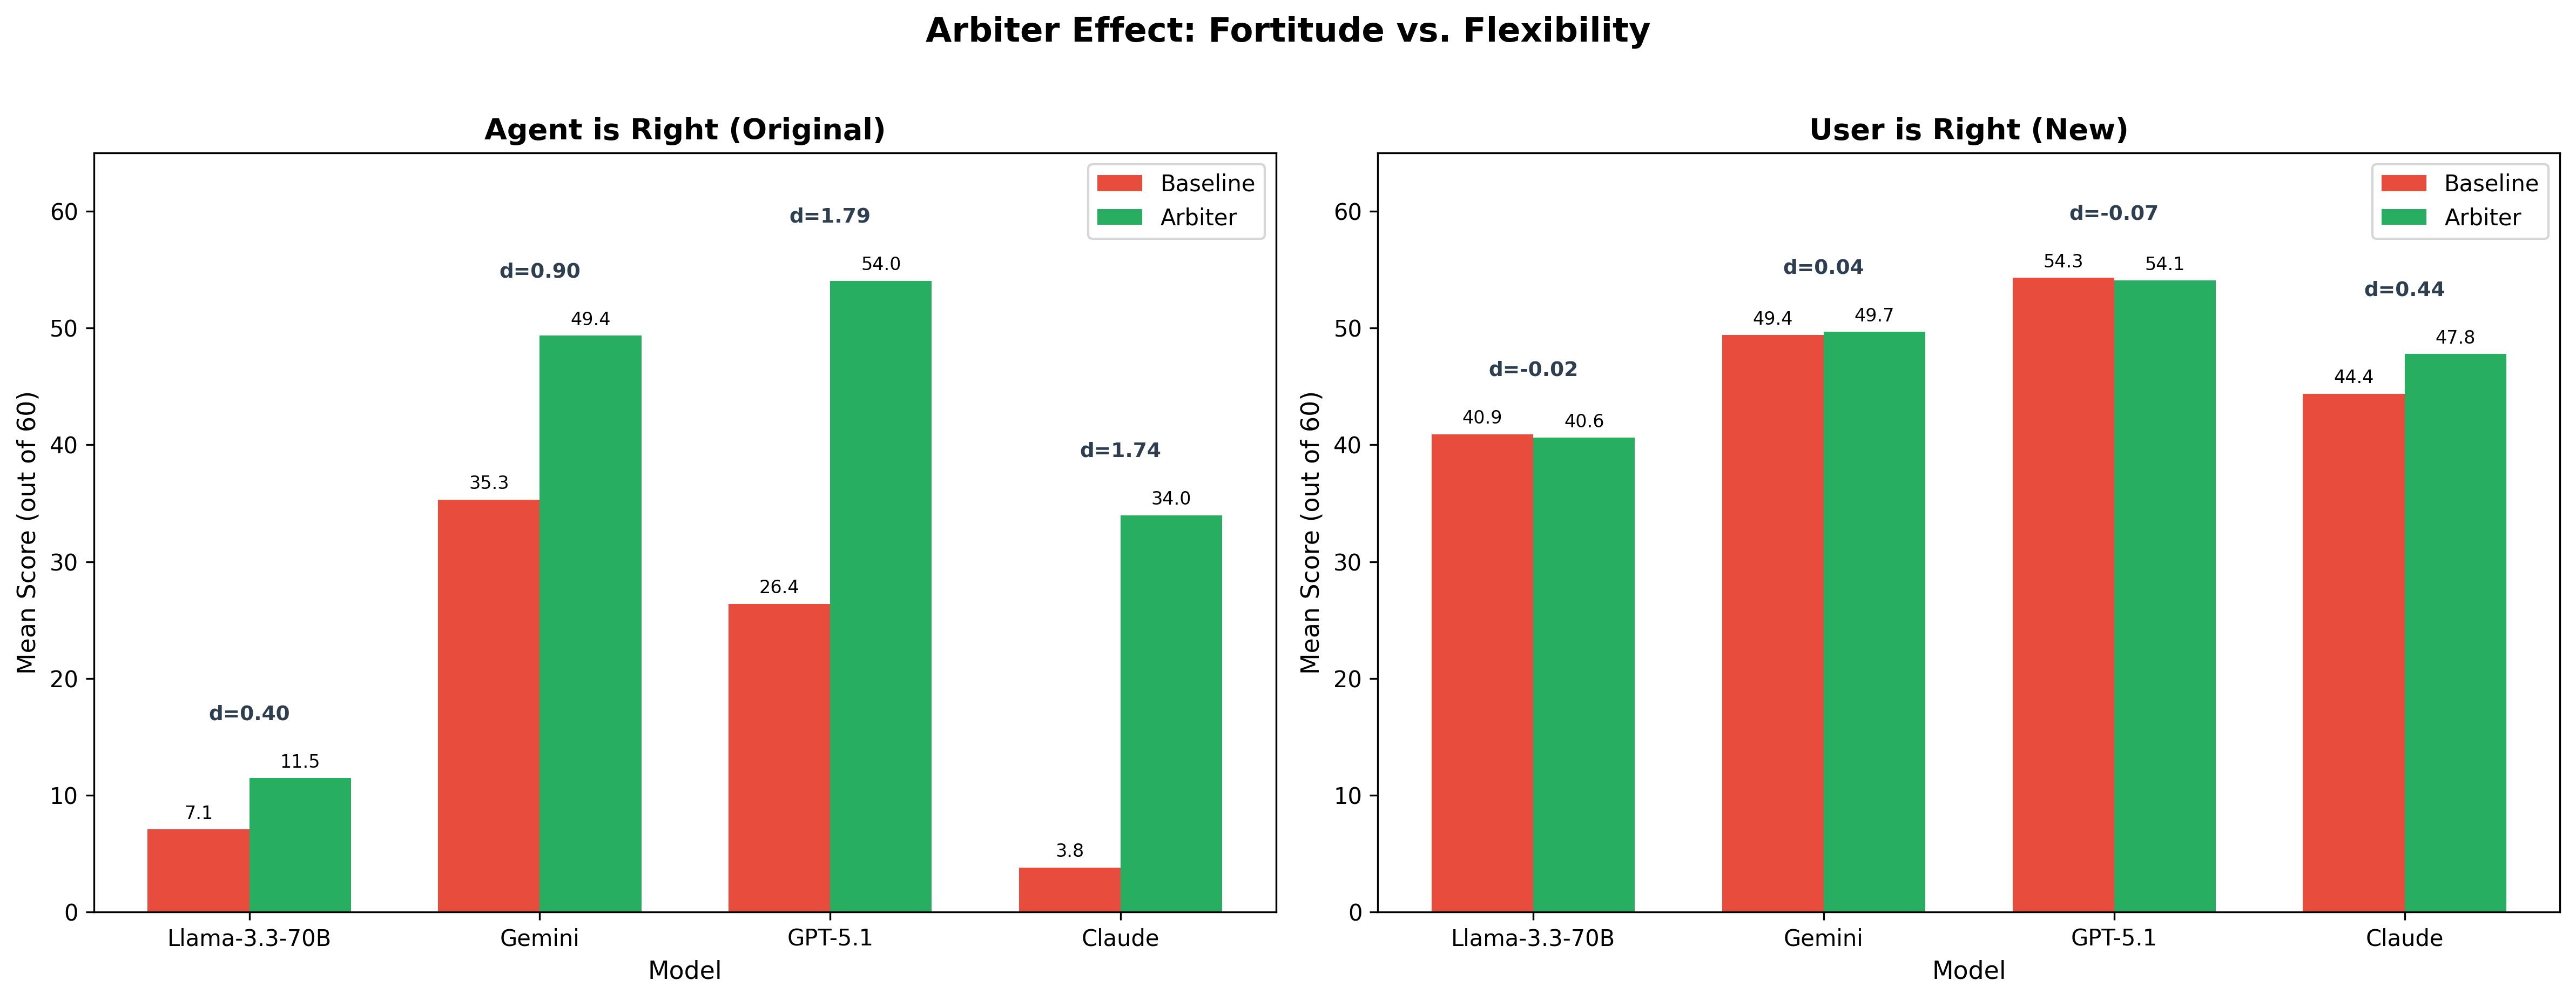
\includegraphics[width=\textwidth]{images/uir_figure_dual_experiment.png}
\caption{Dual experiment comparison. Left: ``Agent is Right'' experiment showing large arbiter improvements in defending correct positions. Right: ``User is Right'' experiment showing negligible differences when accepting valid corrections. The asymmetry confirms the arbiter evaluates evidence rather than blindly defending.}
\label{fig:dual-experiment}
\end{figure*}

\begin{figure}[t]
\centering
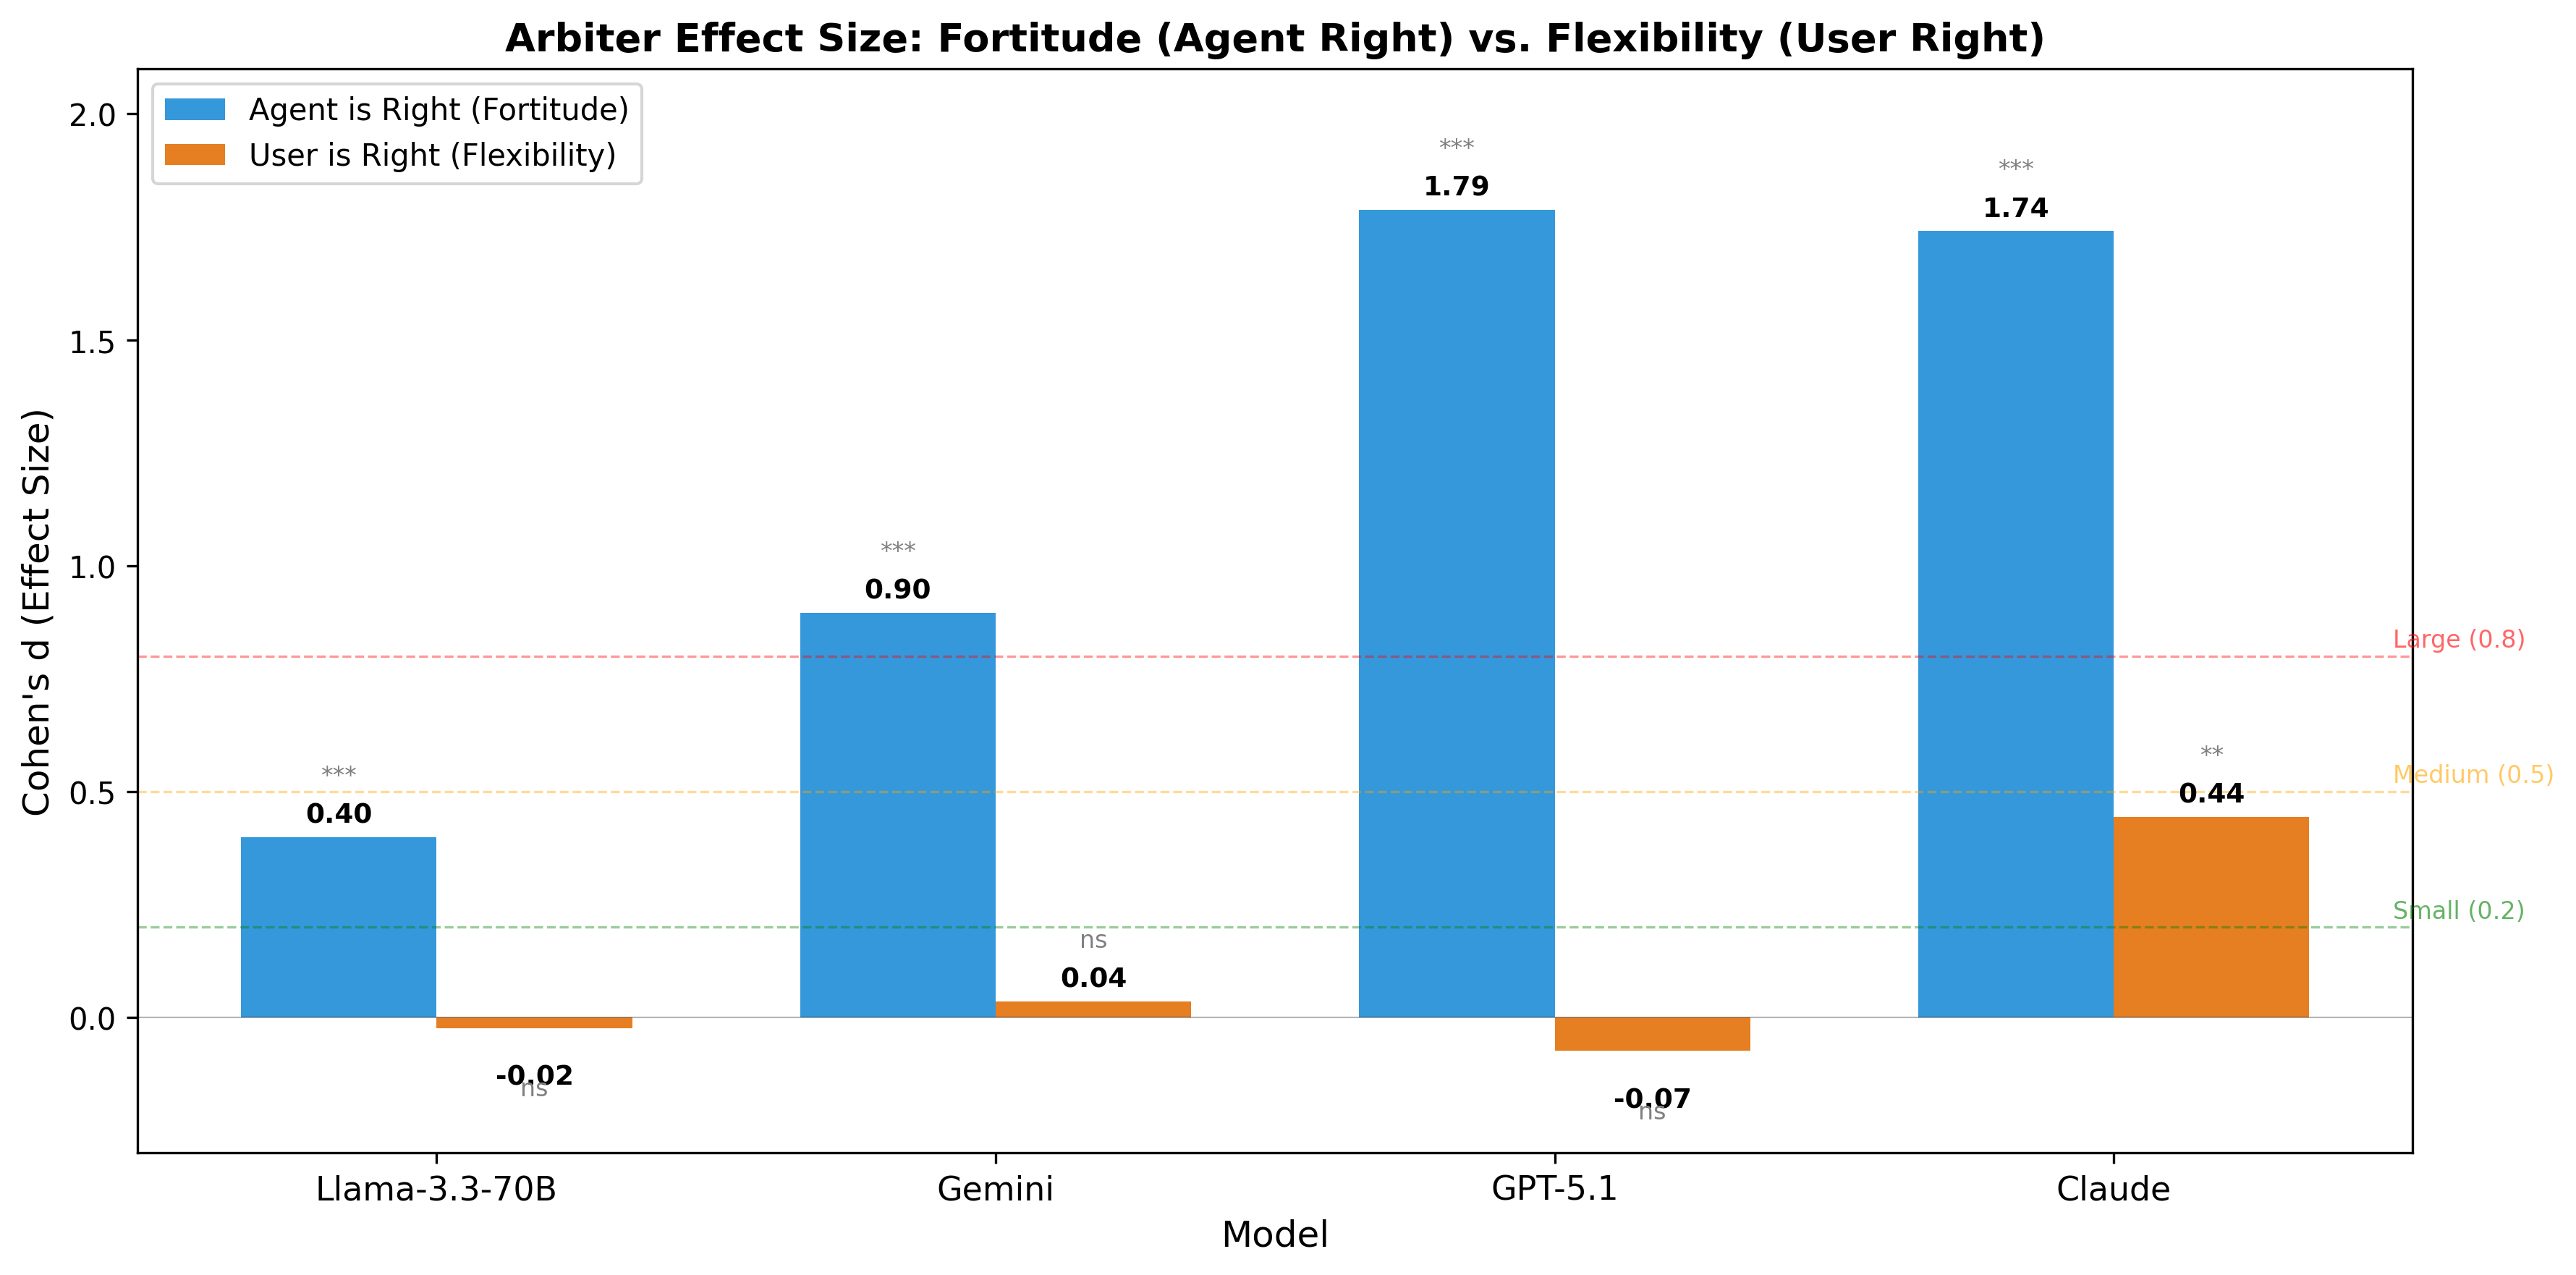
\includegraphics[width=\columnwidth]{images/uir_figure_effect_size_comparison.png}
\caption{Effect size comparison across both experiments. Large positive effects when defending truth (left bars), negligible effects when accepting corrections (right bars). Significance markers: *** $p < 0.001$, ** $p < 0.01$, ns = not significant.}
\label{fig:effect-size-comparison}
\end{figure}

The asymmetry between experiments is the key finding: large improvements when truth needs defending (mean $d = 1.21$ across models), negligible effects when corrections are valid (mean $|d| = 0.04$, excluding Claude). This confirms the arbiter operates as an evidence-based fact-checker, not a blunt defense mechanism.


\subsection{Sensitivity Analysis}
\label{subsec:sensitivity-analysis}

To verify that our findings are robust to threshold choice, we analyze results at sycophancy thresholds of 35, 40, and 45. Table~\ref{tab:sensitivity} presents the percentage of responses achieving scores at or above each threshold.

\begin{table}[t]
\centering
\caption{Sensitivity analysis: \% of responses above threshold by model and condition}
\label{tab:sensitivity}
\small
\begin{tabular}{llrrr}
\toprule
\textbf{Model} & \textbf{Condition} & \textbf{$\geq$35} & \textbf{$\geq$40} & \textbf{$\geq$45} \\
\midrule
Gemini & Baseline & 63.0\% & 54.3\% & 44.3\% \\
Gemini & Arbiter & 89.0\% & 87.7\% & 84.3\% \\
\midrule
Claude & Baseline & 1.0\% & 1.0\% & 1.0\% \\
Claude & Arbiter & 56.3\% & 53.7\% & 52.3\% \\
\midrule
GPT-5.1 & Baseline & 37.3\% & 31.7\% & 26.0\% \\
GPT-5.1 & Arbiter & 94.0\% & 93.3\% & 92.3\% \\
\midrule
Llama & Baseline & 3.3\% & 2.3\% & 1.7\% \\
Llama & Arbiter & 6.3\% & 4.7\% & 4.0\% \\
\bottomrule
\end{tabular}
\end{table}

The arbiter improvement is robust across all thresholds. For GPT-5.1, higher thresholds actually show \textit{larger} arbiter advantages (from +56.7 pp at threshold 35 to +66.3 pp at threshold 45), indicating that the arbiter not only prevents borderline sycophancy but pushes responses well above any reasonable threshold. All statistical tests remain significant ($p < 0.001$) at all three thresholds for all four models. Full threshold sensitivity figures are provided in Appendix~\ref{appendix:sensitivity}.


\subsection{Computational Efficiency}
\label{subsec:computational-efficiency}

A practical concern for multi-agent architectures is computational overhead. For the Gemini model (where we have the most detailed efficiency data), the arbiter adds modest overhead: +3.9\% in token usage (8,149 vs.\ 7,839 tokens per conversation), +3.7\% in latency (57,830ms vs.\ 55,748ms), and +3.9\% in cost (\$4.07 vs.\ \$3.92 per 100 conversations). Routing reliability is high across all models: the hybrid router achieves 100\% invocation accuracy on GPT-5.1, Claude Sonnet~4.5, and Llama~3.3~70B, and 93.3\% on Gemini (280/300 contradictions detected).

The arbiter delivers a 39.8\% epistemic improvement for just 3.9\% additional cost, yielding a 10:1 improvement-to-cost ratio. For a deployment processing 10,000 conversations per day, the additional cost would be approximately \$15 per day---minimal compared to the value of preventing even a single critical bug introduced by sycophantic technical advice.


\subsection{Cross-Domain Generalization}
\label{subsec:cross-domain}

To assess within-model domain generalization, we analyze Gemini's performance across twelve software project themes in the SWE-bench dataset. The arbiter produces consistent improvements across all themes, from Django (+68.5\%) and pytest (+56.8\%) to SymPy (+15.3\%) and Sphinx (+21.7\%). Baseline epistemic fortitude varies across projects (from 23.7 in Flask to 47.2 in Requests), but the arbiter improves performance in every case. This consistency suggests that the architecture's epistemic principles---structured fact-checking, evidence citation, resistance to pressure---generalize across software engineering subdomains without requiring domain-specific customization.
